\documentclass[a4paper, 12pt]{article}

\usepackage[utf8]{inputenc}
\usepackage[T1]{fontenc}
\usepackage[french]{babel} 
\usepackage[top=35mm, bottom=35mm, left=25mm, right=25mm]{geometry}
\usepackage{geometry}
\usepackage{graphicx}
\usepackage{multirow}  
\usepackage{subfigure}
\usepackage{verbatim}
\usepackage{url}
\usepackage{algorithmic, algorithm} 
\usepackage{amsmath,amsfonts,amssymb}
\usepackage{lmodern}
\usepackage{microtype}
\usepackage{xcolor}
\usepackage{textcomp}
\usepackage{minted}
\usepackage{framed}
\usepackage{tcolorbox}
\usepackage{tikz}
\usepackage{pdfpages}
\usepackage{etoolbox}
\graphicspath{{.}}
\begin{document}
    
    
    \begin{center}
    \fbox{ 
    \begin{minipage}[h]{.9\linewidth}
    \begin{center}
    {\vspace*{5mm}
    \huge\textbf{Compte rendu de TP bandit}\\  %%% Titre du rapport
    \vspace*{5mm}}
    \end{center}
    \end{minipage}
    }

    \vspace{15mm}
    {\large 
    \bsc{Chaumette} Noé\\
    \bsc{Sneed} Jérémie}\\
    ~\\
    \underline{STI, 4A}\\ 
    
    \vspace{1cm}  
 
    
    \end{center}
\section{Implémentation et comparaison d'algorithmes bandits}
Après avoir implémenté le pseudo code bandit en python, nous avons 2 expériences différentes afin d'illustrer les points forts et faibles de nos algorithmes. Les 2 expériences ont été réalisées en ayant lancé l'algorithme 100 fois afin d'avoir des résultats représentatifs.
\\Notre première expérience a été efféctuée avec $K = 10$ : 
\[\mu_1=0.4,\mu_2=0.8,\mu_3=0.1,\mu_4=0.2,\mu_5=0.2,\mu_6=0.5,\mu_7=0.7,\mu_8=0.9,\mu_9=0.7,\mu_{10}=0.6\]
Nous avons obtenu les courbes suivantes :\\
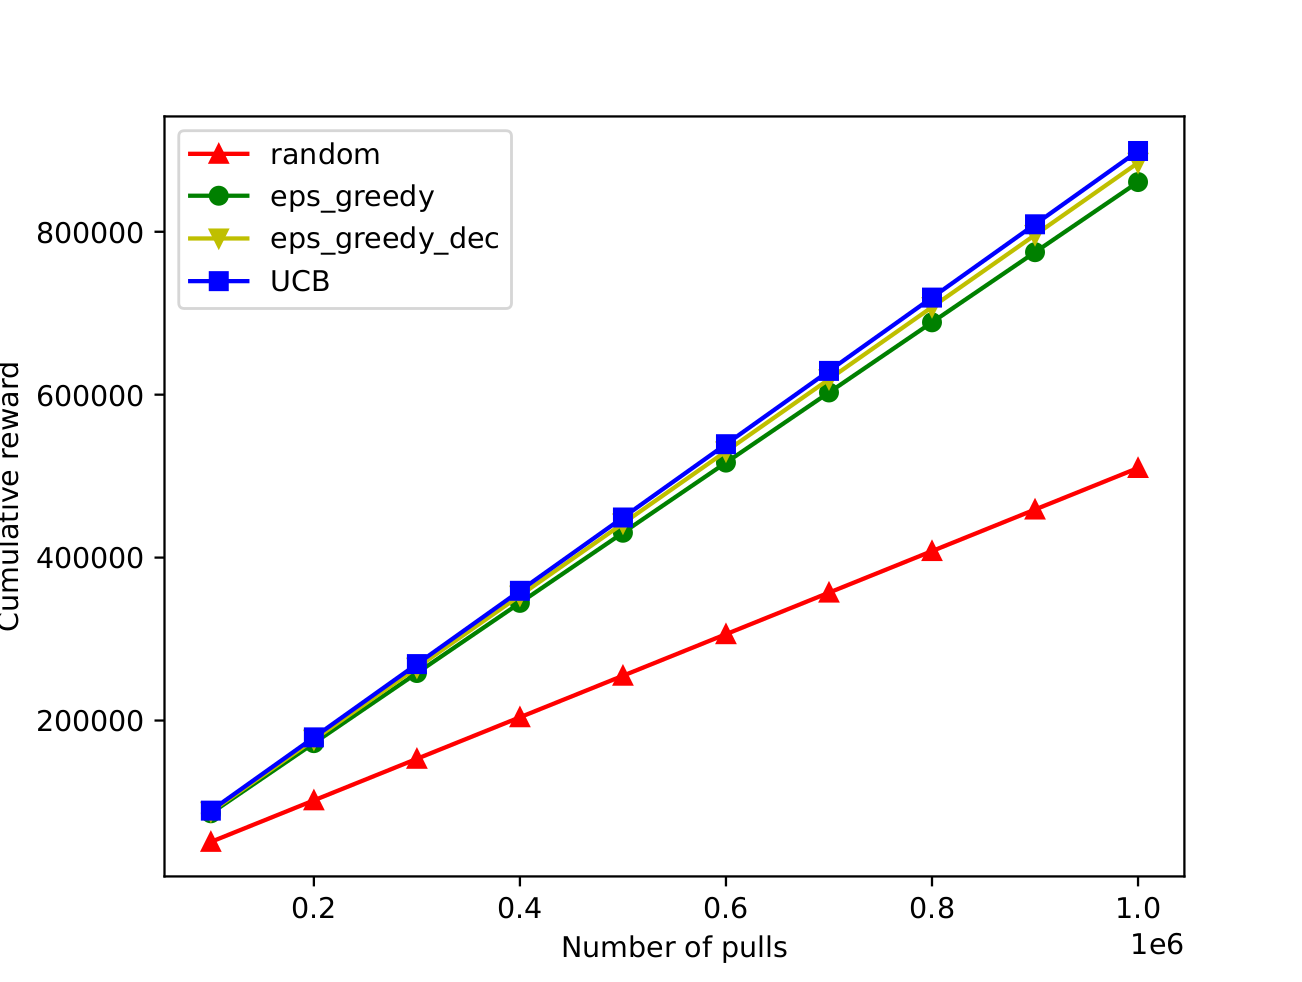
\includegraphics[scale=0.19]{reward_mu_rand.png}
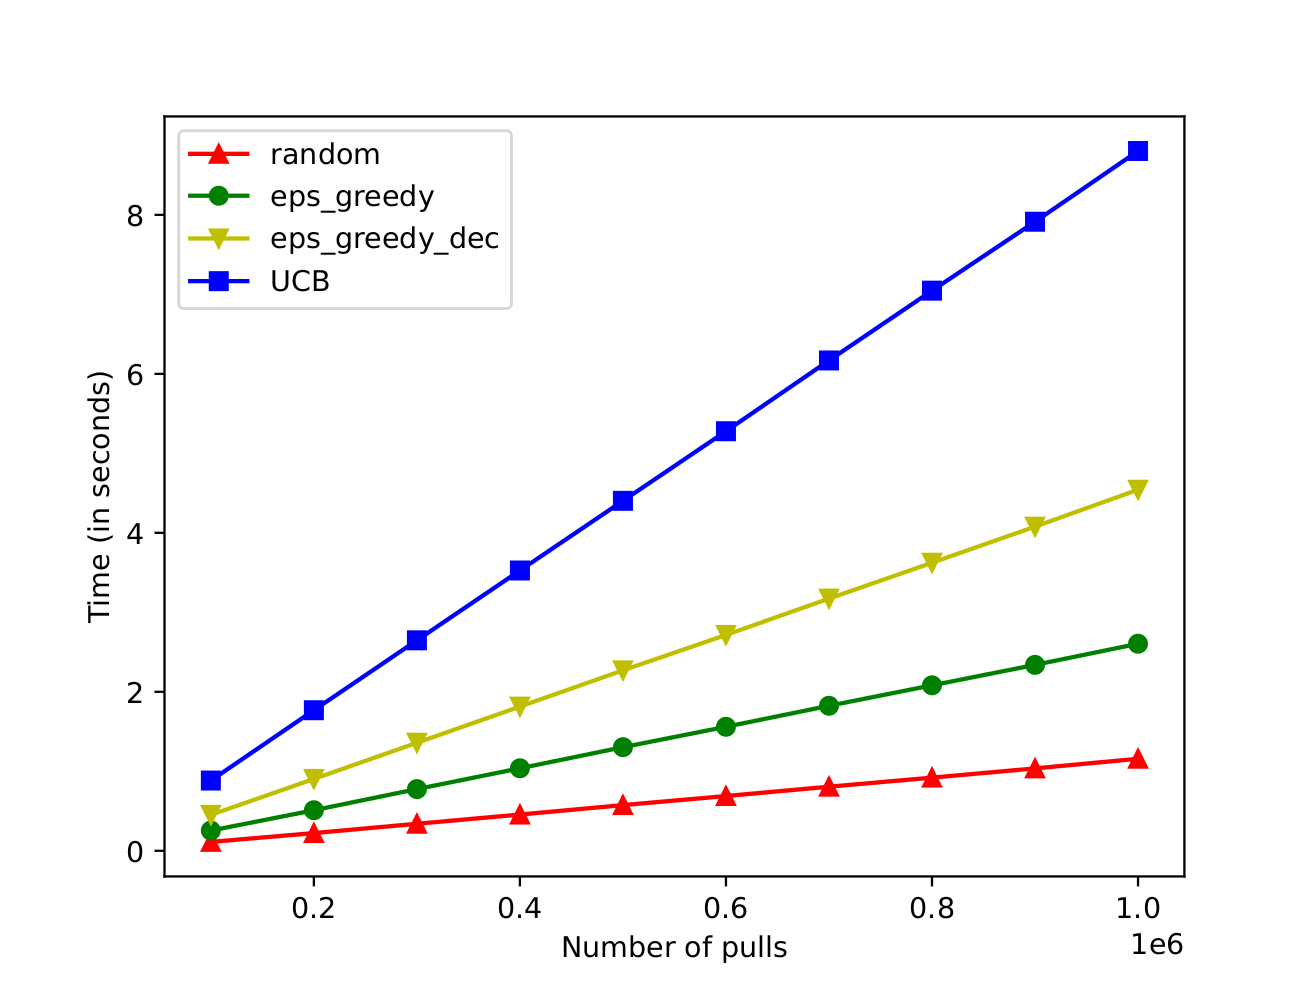
\includegraphics[scale=0.19]{time_mu_rand.png}\\
Notre résultat est cohérent car, pour les récompenses, l'algorithme $\textit{UCB}$ est le plus efficace car le plus rapide à trouver les branches intéressantes afin de les exploiter correctement.
En effet, l'algorithme $\textit{random}$, par exemple, est le plus mauvais car sa stratégie est complétement aléatoire, et, si l'on regarde la moyenne des $\mu$ pour 1000000 d'essais, on a 510000, ce qui correspond au graphique.
Les algorithmes $\epsilon$ et $\epsilon_{dec}$ sont plus efficaces que $\textit{random}$ car ils ont une stratégie d'éxploitation qui leur permet d'optimiser l'appel des branches. 
\\$\epsilon_{dec}$ est meilleur que $\epsilon$ car plus on avance dans les tentatives, plus il va avoir une stratégie d'éxploitation plutôt que d'éxploration, il va donc affiner son utilisation des branches. 
$\textit{UCB}$ est le plus optimal car il va essayer d'éxploiter au maximum, peut-être en négligeant un peu trop l'éxploration. Nous allons voir ça dans notre second cas.
\\\\
Pour notre deuxième expérience, nous avons toujours K = 10 mais des $\mu$ différents :
\[\mu_1=0.1,\mu_2=0.05,\mu_3=0.05,\mu_4=0.01,\mu_5=0,\mu_6=0.1,\mu_7=0.001,\mu_8=0.05,\mu_9=0.15,\mu_{10}=0.02\]
Nous avons obtenu les courbes suivantes :\\
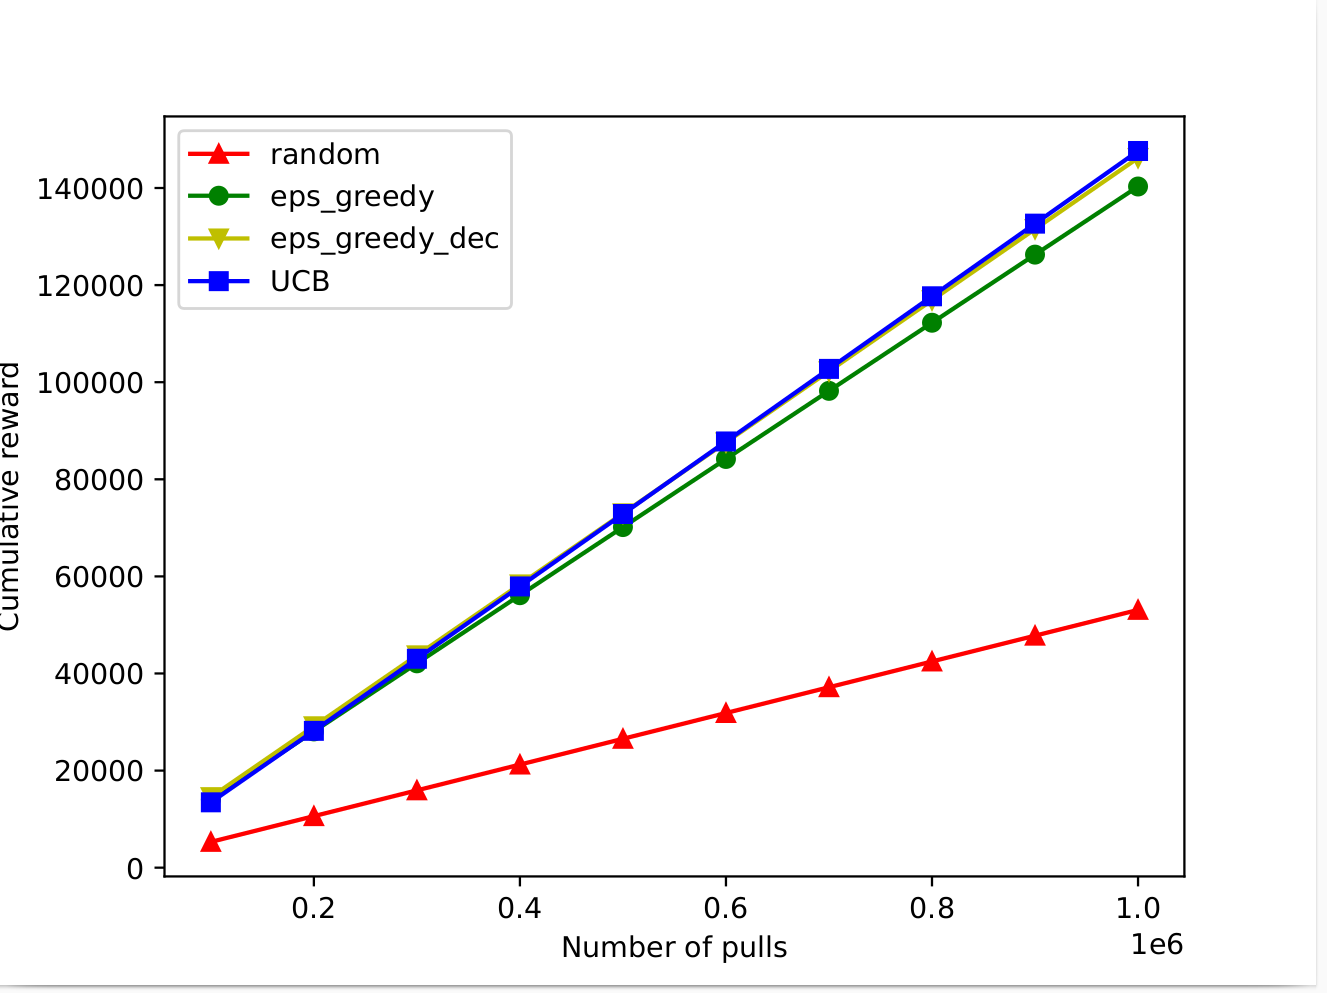
\includegraphics[scale=0.19]{screen_reward_petit_mu.png}
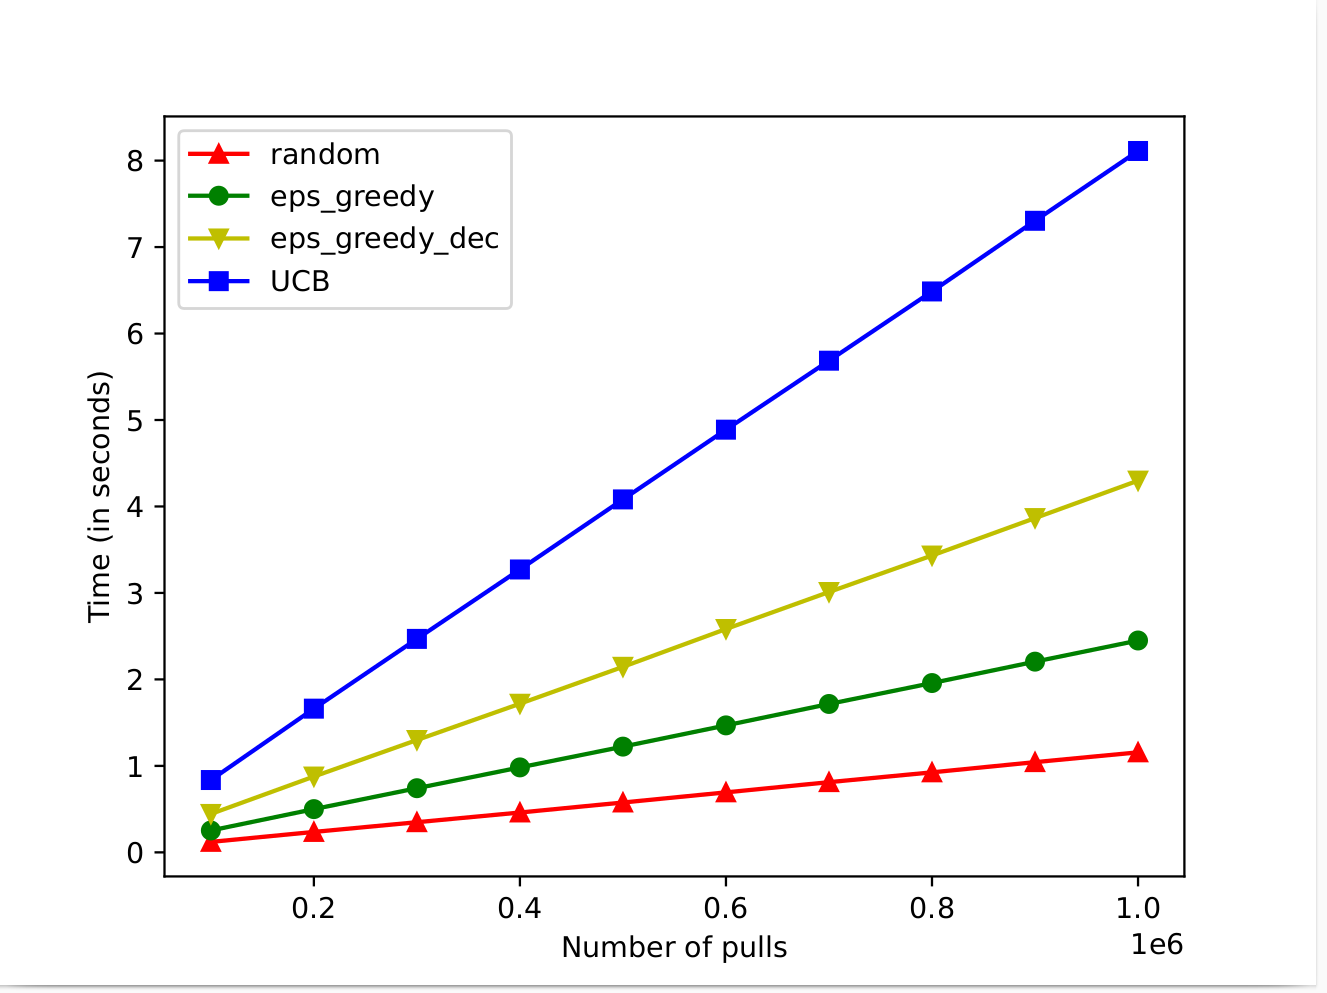
\includegraphics[scale=0.19]{screen_time_petit_mu.png}
Pour ce résultat, l'algorithme $\textit{random}$ est le moins efficace pour les même raison que précédemment. Par contre, l'algorithme $\textit{UCB}$ sera moins efficace car l'utilisation de valeurs très petites et très proches peut désavantager ce dernier par rapport à $\epsilon_{dec}$ ou $\epsilon$.
\\Bien que, globalement, UCB est plus efficace sur la majorité des stratégie par rapport à $\epsilon_{dec}$.
\\Pour le graphique du temps il est tout à fait logique qu'il soit similaire à celui de la précédente stratégie car les valeurs de $\mu$ ne jouent pas sur la compléxité de l'algorithme et donc sur le temps d'éxécution.
\section{Proposition d'un nouveau protocole sécurisé}
\subsection{Présentation de Samba}
Le protocole Sambda est un framework générique pour sécuriser les $multi-armed$ $bandits$. Le principe de base est simple, chaque $data-owner$ possède sa propre distribution des récompenses qui en plus est inconnue des autres.
\\De plus, seul lui peut voir sa récompense cumulée, les autres n'ont accès à aucune information sur lui. Chacun ne peut connaître des informations que sur eux même.
\\Le protocole Samba est très utile car il peut utiliser de nombreux algorithmes bandits standatds (comme UCB par exemple) et c'est un protocole sécurisé à l'aide de cryptographie (AES en général mais cela peut varier). 
\\Pour plus de détails, le score va être encrypté par le $data-owner$ et être envoyé au controlleur. Ce controlleur va créer une nouvelle liste avec le texte encrypté et va envoyer la liste permutée à $comp$. 
Comp sera capable de décrypter chaque text et va créer une liste remplie de 0, sauf à la case $i$ qui devra être $pull$. Il va envoyer cette liste au controlleur qui va la dépermuter et donner chaque récompenses aux bonnes personnes.

\subsection{Nouveau protocole sécurisé}
Nous pouvons imaginer un nouveau protocole basé sur de l'isolation (en utilisant la technologique de $\mu$-noyau par exemple).
\\En effet, ce protocole aurait un $controlleur$ qui pourrait créer un nouveau $controlleur$ pour chaque $data-owner$. Chaque $controlleur$ associé aurait la distribution personnalisé du $data-owner$ un peu comme pour le Samba.
\\ Ainsi, les $data-owners$ ne seront pas du tout en contact avec les controlleur des autres, ils seront donc isolés. 
\\De plus, pour protéger des packets sniffer, les données seront encryptés en utilisant un algorithme performant comme AES par exemple. Seul le controlleur originel sera en lien avec un decrypteur qui lui permettra d'analyser les résultats et de continuer l'algorithme.
\\Pour plus de détails voici un schéma explicatif :\\
\begin{center}
    \begin{tikzpicture}
        \node[draw, circle] (Decrypter) at (-3,0) {Decrypter};
        \node[draw, circle] (Controller) at (2,0) {Controller};
        \node[draw, circle] (V-Controller-1) at (-4.5,-4) {V-Controller-1};
        \node[draw, circle] (V-Controller-2) at (-1,-4) {V-Controller-2};
        \node[draw, circle] (V-Controller-3) at (2.5,-4) {V-Controller-3};
        \node[draw, circle] (V-Controller-4) at (6,-4) {V-Controller-4};
        \node[draw, circle] (Data-Owner-1) at (-4.5,-7.5) {Data-Owner-1};
        \node[draw, circle] (Data-Owner-2) at (-1,-7.5) {Data-Owner-2};
        \node[draw, circle] (Data-Owner-3) at (2.5,-7.5) {Data-Owner-3};
        \node[draw, circle] (Data-Owner-4) at (6,-7.5) {Data-Owner-4};
        
        
        \draw (Decrypter) -- (Controller);
        \draw (V-Controller-1) -- (Data-Owner-1);
        \draw (V-Controller-2) -- (Data-Owner-2);
        \draw (V-Controller-3) -- (Data-Owner-3);
        \draw (V-Controller-4) -- (Data-Owner-4);
        \draw[dash pattern=on 3pt off 3pt] (Controller) -- (V-Controller-1);
        \draw[dash pattern=on 3pt off 3pt] (Controller) -- (V-Controller-2);
        \draw[dash pattern=on 3pt off 3pt] (Controller) -- (V-Controller-3);
        \draw[dash pattern=on 3pt off 3pt] (Controller) -- (V-Controller-4);
    \end{tikzpicture}
\end{center}
Nous avons donc les V-Controller qui sont les controlleurs virtuels séparés par le $\mu$-noyau afin d'avoir des processus complétement isolés pour chaque data owner. 
Et la partie de decryptage avec le controlleur originel afin qu'il puisse décrypter ce qu'il reçoit afin de l'analyser.
Petite précision, nous ne connaissons pas la validité exacte de notre système et s'il est réellement viable. Mais nous espérons qu'il puisse l'être.
\end{document}